Considering that Mold \& Co's new production plant implies an important
and complex system, we have to identify and evaluate all the risks
inherent to this system in order to limit them the most possible. This
risk analysis will allow us to help designing the new production system
by establishing the most efficient preventive and correctives measures.

In order to deal with the risk management, we decided to use the FMECA
Method on the means of production of Mold \& Co company. This means that
we consider all the risks related to the operation of the assembly line
system.

\subsection{Plan}

For that purpose, we have to, as a first step, describe the overall
production system. Then we will be able to identify all the threats.
After this step, we will identify all the threats that could affects the
system and assess them in order to define their criticality.

Ultimately, we will see how to compensate these eventual failure modes
where appropriate.

\subsection{Description of the system}

The assembly line system is composed of two main parts : the mechanical
system and the computing's one.

By the way, we estimate that these two systems are interdependent. In
other words, we have to take into account that if the mechanical part of
the assembly line fails, the entire system cannot work anymore and vice
versa.

Actually, mechanical part of the production chain can work independently
but if the computing system is not working, the mechanical will
encounter problems about its regulation and monitoring.

\subsection{Definition of the risk assessment}

According to the FMECA Method, we have to assess three different values
in the table of risk.

First of all, the Severity (S) which equals to the importance of the
consequences that the risk could induce on the production of the
factory. More the risk can affect the production line, more the Severity
level is high as the following table shows :

\begin{figure}[h]
    \centering
    \begin{tabular}{| p{4cm} | c | c |}
        \hline
        \rowcolor{heading-color}\multicolumn{1}{|c|}{Severity definition} & Severity level & Associated color\\
        \hline
        Insignificant & 1 & green  \\
        \hline
        Minor & 2 & light green  \\
        \hline
        Significant & 3 & yellow  \\
        \hline
        Serious & 4 & orange  \\
        \hline
        Major & 5 & red  \\
        \hline
    \end{tabular}
    \caption{Table of severity level}
\end{figure}

Then we have to assess the Occurrence (O) of the risks. The occurrence enables us to measure the likelihood of the risk. Mire the risk is potential, more the Occurrence value is high as we can see as below :

    \begin{figure}[h]
        \centering
        \begin{tabular}{| p{4cm} | c | c |}
            \hline
            \rowcolor{heading-color}\multicolumn{1}{|c|}{Occurrence definition} & Occurrence level & Associated color\\
            \hline
            Remote & 1 & green  \\
            \hline
            Very low & 2 & light green  \\
            \hline
            Low & 3 & yellow  \\
            \hline
            Moderate & 4 & orange  \\
            \hline
            Major & 5 & red  \\
            \hline
        \end{tabular}
        \caption{Table of occurence level}
\end{figure}

Finally, the Detection (D) is measured according to the ease for the operators to discover a failure mode. As we can see on the below table, higher the value is, harder it is to detect the issue.

\begin{figure}[h]
    \centering
    \begin{tabular}{| p{4cm} | c |}
        \hline
        \rowcolor{heading-color}\multicolumn{1}{|c|}{Detection definition} & Detection level\\
        \hline
        Blatant & 1  \\
        \hline
        Easily identifiable & 2  \\
        \hline
        Discreet & 3  \\
        \hline
        Hard to identify & 4 \\
        \hline
        Very  hard to identify & 5 \\
        \hline
    \end{tabular}
    \caption{Table of detection level}
\end{figure}

\subsection{Calculation of the criticality and risk priority numbers}

In sum, Severity, Occurrence and Detection are arbitrarily assessed whereas Criticality and RPN are calculated from these same data.\\

Especially, we have the following relations :
\begin{itemize}
    \item Criticality = Severity \* Occurrence
    \item RPN = Severity \* Occurrence \* Detection = Criticality \* Detection
\end{itemize}

These last two measures enable us to prioritize the risk in order to make the further effort in order to limit them and eventually resolve them if ever they occur.

\section{Calculation of the criticality and risk priority numbers}

In sum, Severity, Occurrence and Detection are arbitrarily assessed
whereas Criticality and RPN (Risk Priority Number) are calculated from these same data.

Especially, we have the following relations :

\[Criticality = Severity \times Occurrence\]
\[RPN = Severity \times Occurrence \times Detection = Criticality \times Detection\]

These last two measures enable us to prioritize the risk in order to
make the further effort in order to limit them and eventually resolve
them if ever they occur.

\begin{figure}[h]
\centering
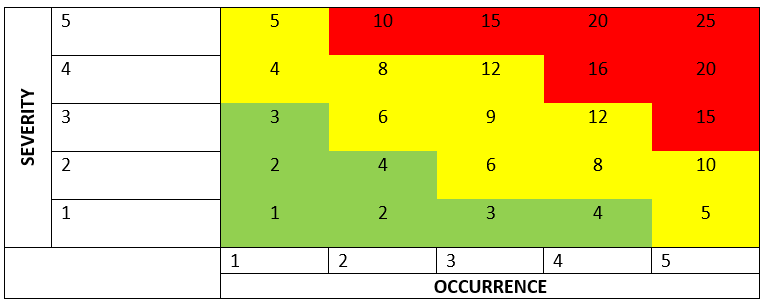
\includegraphics[scale=0.7]{Img/severity-occurrence.png}
\caption{Severity occurences}
\end{figure}

After having defined all the measure required in order to assess the risks. We can now list them,  

evaluate their Severity (S), Occurrence (O), Detection (D) and thus calculate for each one, their criticality (C) and their Risk Priority Number (RPN). 

\begin{landscape}
\begin{figure}[h]
\centering
\resizebox{\textwidth}{!}{%
\begin{tabular}{|l|p{3cm}|p{3cm}|p{3cm}|p{3cm}|p{3cm}|l|l|l|l|l|}
\hline
Identifier & Failure mode               & Failure causes                     & Failure effect                      & Detection method                  & Corrective actions                                & S & O & D & C  & RPN \\
\hline
A          & Power outage               & Equipment disfunction              & Stop of the production              & Beep                              & Inverter and external batteries                   & 5 & 4 & 1 & 20 & 20  \\
\hline
B          & Noise pollution            & Equipment disruption               & Employee’s discomfort               & Error message                     & Automatic measurement and earplugs                & 1 & 2 & 2 & 2  & 4   \\
\hline
C          & Inherent materiel defect   & Obsolescence                       & Slowdown or stop of the production  & Error message                     & Periodic maintenance                              & 5 & 4 & 2 & 20 & 40  \\
\hline
D          & Earthquake                 & Environment                        & Stop of the production              & Sound and tremors                 & Earthquake protection                             & 4 & 1 & 1 & 4  & 4   \\
\hline
E          & Fire                       & Overheat                           & Stop of the production              & Beep (fire alarm), flames         & Fire prevention system                            & 4 & 1 & 1 & 4  & 4   \\
\hline
F          & Lack of raw materials      & Desynchronization                  & Stop of the production              & Alert message                     & Provider proximity and Daily stock’s review       & 4 & 2 & 1 & 8  & 8   \\
\hline
G          & Short circuit              & Equipment disfunction              & Slowdown or stop of the production  & Alert message                     & Circuit-breakers                                  & 4 & 3 & 1 & 12 & 12  \\
\hline
H          & Absence of a main operator & Leave                              & Relative stop of the production     & Control presence of the employees & Control presence of the employees                 & 3 & 4 & 1 & 12 & 12  \\
\hline
I          & Local network outage       & Broken cable                       & Stop of the production              & Error message                     & Network connection cable redundancy               & 5 & 5 & 1 & 25 & 25  \\
\hline
J          & Lightning                  & Environment                        & None                                & Lightning sound                   & Lightning rod                                     & 1 & 1 & 1 & 1  & 1   \\
\hline
K          & Flood                      & Water leak                         & Eventual stop of the production     & Leak detectors                    & Water recycling system                            & 2 & 3 & 1 & 6  & 6   \\
\hline
L          & Over-voltage               & Insulation failure                 & Stop of the production              & Alert message                     & Circuit-breakers                                  & 4 & 2 & 1 & 8  & 8   \\
\hline
M          & Vandalism                  & Human error                        & Slowdown or stop of the production  & Cameras                           & Cameras and Intern investigation                  & 4 & 2 & 2 & 8  & 16  \\
\hline
N          & Overload                   & Equipment dysfunction (disruption) & Slowdown or stop of the production  & Error message                     & Regular control of the equipment’s settings       & 4 & 3 & 2 & 12 & 24  \\
\hline
O          & Product quality defect     & Human error                        & Slowdown of the production          & Block of the equipment            & Regular quality controls                          & 2 & 3 & 1 & 6  & 6   \\
\hline
P          & Environmental pollution    & Equipment dysfunction (disruption) & Penalty                             & Pollution traces                  & Regular analysis on the water and other resources & 3 & 3 & 3 & 9  & 27  \\
\hline
Q          & Non respect of deadlines   & Wrong estimation of the delays     & Economic losses                     & Project management                & Recursive estimation                              & 3 & 5 & 2 & 15 & 30  \\
\hline
R          & Employee’s injury          & Accident                           & Eventual slowdown of the production & Complain                          & None                                              & 3 & 1 & 1 & 3  & 3  \\
\hline
\end{tabular}%
}
\caption{Risk table}
\end{figure}
\end{landscape}

\begin{figure}[h]
    \centering
    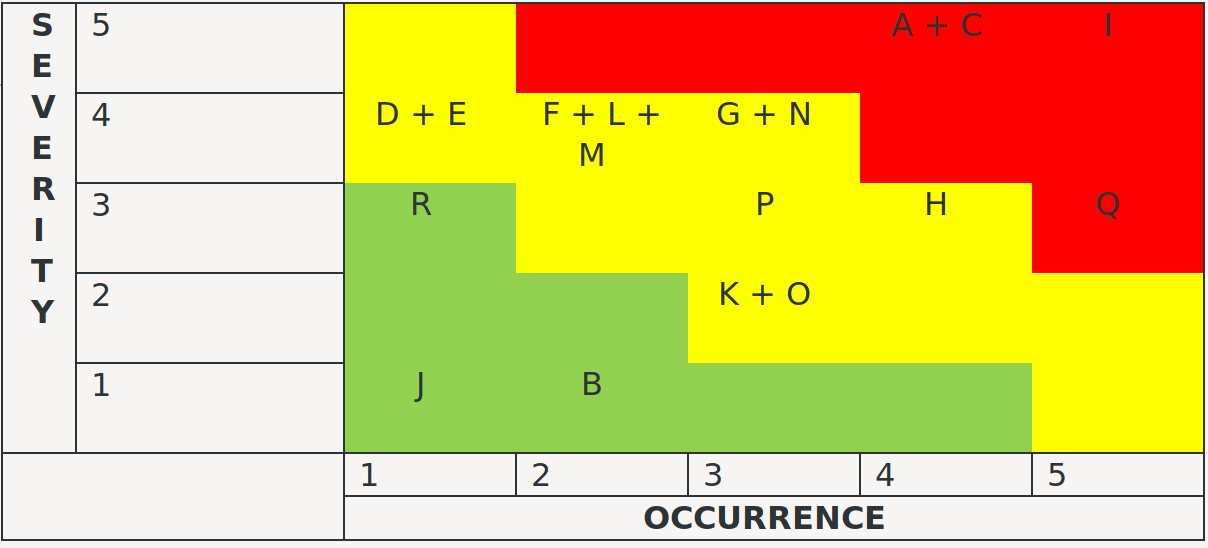
\includegraphics[scale=0.3]{Img/severity.png}
    \caption{Table of severity}
\end{figure}

\subsection{Prevention and correction of the risks}

What we can conclude from this table is that four risks : A, C, I and Q
are particularly important as their criticality is in the red color so
high priority.

Then we have to pay a special attention to these one and foresee strong
corrective actions in order not only for prevention but also for
correction.

Particularly, for these risk we decided to :

\begin{itemize}
\item
  Power outage (A) : provide external batteries while the failure is not
  resolved
\item
  Inherent materiel defect (C) : plan periodic maintenance on all the
  different machine consisting in verifying all its functionalities
\item
  Local network outage (I) : foresee a double connection on the machines
  for the local network so that if one is defaulting, the other will
  relay the connection
\item
  Non respect of the deadlines (Q) :

  \begin{itemize}
  \item
    foresee provisional timeline of 10\% of the time required to achieve
    the project
  \item
    daily checks of the projects progress
  \end{itemize}
\end{itemize}
